\chapter{Thực nghiệm}
Trong quá trình thực nghiệm, nhóm tập trung vào việc đánh giá hiệu quả của mô hình đề xuất so với các backbone khác (ResNet-50, CLIP, MedCLIP, BiomedCLIP, PubMedCLIP) trên nhiệm vụ phân loại ảnh x-quang. Nhóm đã thiết lập một loạt các thí nghiệm để so sánh hiệu suất của các mô hình này, đồng thời thực hiện các thí nghiệm rời rạc để kiểm tra ảnh hưởng của việc sử dụng thông tin văn bản, các đóng góp của các thành phần đề xuất trong quá trình huấn luyện và đánh giá.

\section{Mục đích thực nghiệm}
Nhằm chứng minh cho các luận điểm mà nhóm đưa ra, đóng góp lý thuyết cũng như thực tiễn của mô hình đề xuất XBone-Net trên bài toán hỗ trợ chẩn đoán và phân loại đa lớp ảnh x-quang xương, nhóm nghiên cứu đã thiết lập một hệ thống các thí nghiệm thực nghiệm. Mỗi thí nghiệm được xây dựng nhằm xác thực một luận điểm cụ thể, giải quyết các thách thức của bài toán phân loại ảnh x-quang xương đa phương thức và kiểm chứng các cải tiến về mặt kiến trúc cũng như phương pháp huấn luyện hai pha.

\subsection{Đánh giá so sánh hiệu năng chẩn đoán với các mô hình đối sánh}
Mục đích chính của nhóm thí nghiệm này là đặt mô hình đề xuất XBone-Net vào mối tương quan so sánh trực tiếp với các mô hình học sâu đa phương thức y khoa hiện nay. Các mô hình đối sánh được lựa chọn bao gồm cả kiến trúc đơn phương thức truyền thống như ResNet-50 và các mô hình ngôn ngữ trực quan mạnh mẽ như CLIP, MedCLIP, BiomedCLIP và PubMedCLIP. Thí nghiệm này nhằm chứng minh các luận điểm sau:
\begin{itemize}
    \item Sự vượt trội của việc kết hợp thông tin đa phương thức (ảnh chụp X-quang và văn bản bệnh sử lâm sàng) so với các phương pháp chỉ sử dụng thông tin hình ảnh thị giác đơn thuần trong việc phân biệt các lớp bệnh lý u xương có hình thái tương đồng trên ảnh x-quang.
    \item Hiệu quả vượt trội của việc sử dụng các mô hình ngôn ngữ trực quan y khoa tiền huấn luyện làm bộ trích xuất đặc trưng so với các mô hình ngôn ngữ trực quan tiền huấn luyện trên dữ liệu ảnh tự nhiên nói chung, do sự thu hẹp khoảng cách miền dữ liệu.
    \item Khả năng tối ưu hóa vượt trội của mô hình đề xuất XBone-Net trong việc duy trì độ chính xác cao trên toàn cục đồng thời bảo toàn độ nhạy chẩn đoán đối với các lớp bệnh lý hiếm gặp trong bối cảnh mất cân bằng dữ liệu.
\end{itemize}

\subsection{Đánh giá khả năng phát hiện dữ liệu ngoài phân phối}
Trong môi trường lâm sàng thực tế, mô hình phân loại có thể phải đối mặt với các hình ảnh X-quang không chứa khối u xương mà chứa các loại bệnh lý xương khớp khác (như gãy xương, viêm khớp, loãng xương) hoặc ảnh chụp từ các vùng giải phẫu không liên quan. Mục đích của thí nghiệm này là đánh giá độ tin cậy và an toàn y khoa của mô hình thông qua khả năng phát hiện dữ liệu ngoài phân phối thay vì đưa ra các chẩn đoán sai lệch. Thí nghiệm hướng đến việc kiểm chứng giả thuyết:
\begin{itemize}
    \item Việc sử dụng đầu phân loại nguyên mẫu kết hợp học khoảng cách ở Pha 2 giúp tạo lập một không gian đặc trưng có cấu trúc cụm chặt chẽ hơn.
    \item Độ tương đồng cosine giữa vector đặc trưng của mẫu kiểm thử với các nguyên mẫu của lớp đã biết cung cấp một thước đo khoảng cách đáng tin cậy để xác định ranh giới từ chối chẩn đoán, giúp phát hiện các mẫu ngoài phân phối.
\end{itemize}

\subsection{Đánh giá vai trò của các nguồn thông tin văn bản lâm sàng}
Thông tin văn bản y khoa có thể đến từ nhiều nguồn khác nhau trong quy trình chẩn đoán lâm sàng. Thí nghiệm này được thiết lập nhằm bóc tách đóng góp cụ thể của từng nguồn văn bản (báo cáo mô tả hình ảnh X-quang và báo cáo lâm sàng) đến kết quả phân loại cuối cùng. Mục đích cốt lõi của thí nghiệm này bao gồm:
\begin{itemize}
    \item Phát hiện và ngăn chặn hiện tượng rò rỉ nhãn trong học máy đa phương thức y tế. Các báo cáo chẩn đoán X-quang cận lâm sàng thường chứa trực tiếp tên của bệnh lý (ví dụ: "osteosarcoma"). Nếu đưa báo cáo này vào huấn luyện, mô hình sẽ học cách đọc trực tiếp từ khóa này thay vì phân tích các dấu hiệu thị giác trên ảnh, dẫn đến việc mất đi giá trị chẩn đoán thực tế khi ứng dụng.
    \item Khẳng định giá trị lâm sàng thực tế của báo cáo tổng quát như tuổi tác, giới tính, vị trí sưng đau, tiền sử bệnh án. Đây là nguồn thông tin an toàn, không gây rò rỉ nhãn và đóng vai trò hỗ trợ đắc lực cho hình ảnh X-quang để đưa ra kết luận chẩn đoán chính xác nhất.
\end{itemize}

\subsection{Đánh giá ảnh hưởng của chiến thuật tinh chỉnh backbone}
Mục đích của nhóm thí nghiệm này là nghiên cứu và so sánh các chiến thuật cập nhật trọng số cho các bộ trích xuất đặc trưng bao gồm: đóng băng hoàn toàn, tinh chỉnh hiệu quả tham số và tinh chỉnh toàn bộ. Nhóm thí nghiệm hướng tới chứng minh hai luận điểm quan trọng:
\begin{itemize}
    \item \textbf{Hiện tượng quên biểu diễn:} Xảy ra khi có sự không đồng nhất về mặt ngữ nghĩa giữa nguồn thông tin văn bản được sử dụng trong Pha 1 học biểu diễn và Pha 2 học phân loại. Thí nghiệm nhằm chứng minh việc đồng bộ hóa nguồn văn bản lâm sàng ở cả hai pha sẽ bảo toàn không gian biểu diễn chung, tránh trôi lệch đặc trưng và nâng cao đáng kể hiệu năng chẩn đoán.
    \item \textbf{Quên tri thức gốc và Quá khớp:} Thí nghiệm kiểm chứng giả thuyết rằng việc áp dụng PEFT (QLoRA) kết hợp với quy trình huấn luyện hai pha sẽ giúp giữ lại các tri thức y khoa nền tảng mạnh mẽ đã học được ở giai đoạn tiền huấn luyện trên bộ dữ liệu quy mô lớn, ngăn chặn hiện tượng quên đặc trưng khi tinh chỉnh trên tập dữ liệu y sinh nhỏ so với Full Fine-Tuning.
\end{itemize}

\subsection{Đánh giá hiệu quả của đầu phân loại nguyên mẫu so với đầu phân loại tuyến tính}
Thí nghiệm này tập trung vào việc đánh giá so sánh hiệu năng của đầu phân loại nguyên mẫu, sử dụng khoảng cách để phân lớp, so với đầu phân loại tuyến tính truyền thống. Mục đích thực nghiệm là xác minh:
\begin{itemize}
    \item Khả năng xây dựng ranh giới quyết định của phân loại nguyên mẫu trong không gian đặc trưng.
    \item Sự ổn định và khả năng chống chịu của đầu phân loại nguyên mẫu khi đối mặt với hiện tượng trôi lệch biểu diễn hoặc nhiễu dữ liệu. Bằng cách định hướng quá trình tối ưu kéo gần các đặc trưng cùng lớp về phía nguyên mẫu đại diện và đẩy xa các lớp khác thông qua hàm loss khoảng cách có khoảng lề, phân loại nguyên mẫu giúp ổn định ranh giới quyết định tốt hơn đầu tuyến tính.
\end{itemize}

\subsection{Trực quan hóa bản đồ chú ý chéo và khả năng giải thích y khoa}
Thí nghiệm này nhằm trực quan hóa các vùng chú ý của mô hình khi đưa ra quyết định phân loại, từ đó cung cấp khả năng giải thích lâm sàng và tính minh bạch cho các dự đoán của mô hình đề xuất XBone-Net. Mục đích thực nghiệm cụ thể bao gồm:
\begin{itemize}
    \item \textbf{Đánh giá khả năng định vị tổn thương giải phẫu:} Xác minh xem vùng tập trung chú ý cao nhất của bản đồ chú ý chéo trích xuất từ mô-đun Cross-Attention Fusion có thực sự trùng khớp với phân vùng tổn thương thực tế được chú thích bởi các chuyên gia y tế trên ảnh X-quang hay không.
    \item \textbf{Kiểm chứng tương tác đa phương thức:} Chứng minh rằng thông tin từ bệnh sử lâm sàng dạng văn bản đóng vai trò dẫn đường hiệu quả, giúp mô hình tập trung vào các vùng giải phẫu đặc trưng của từng bệnh cảnh cụ thể trên ảnh X-quang, thay vì dựa vào các chi tiết nền không liên quan.
    \item \textbf{Củng cố độ tin cậy trong hỗ trợ chẩn đoán:} Chứng minh tính hợp lý về mặt y học của ranh giới quyết định, giúp các bác sĩ hiểu rõ cơ sở logic của mô hình khi đưa ra dự đoán chẩn đoán, từ đó tăng cường độ tin cậy trong các ứng dụng thực tế.
\end{itemize}

\section{Chuẩn bị dữ liệu}
Để minh chứng hiệu quả của mô hình đề xuất, nhóm đã sử dụng hai tập dữ liệu xương được thu thập từ bệnh viện chấn thương chỉnh hình và bộ dữ liệu BTXRD được công bố \cite{Yao2025}. Các tập dữ liệu này bao gồm các hình ảnh xương cùng với các nhãn và mô tả bệnh lý tương ứng. Nhóm đã thực hiện các bước tiền xử lý dữ liệu, bao gồm chuẩn hóa hình ảnh và mã hóa nhãn, để đảm bảo tính nhất quán và chất lượng của dữ liệu trước khi đưa vào quá trình huấn luyện và đánh giá mô hình.

\subsection{Bộ dữ liệu BTXRD}
Bộ dữ liệu hình ảnh X-quang U xương (Bone Tumor X-ray Radiograph dataset - BTXRD) được xây dựng nhằm hỗ trợ cho các nghiên cứu về phân loại, định vị và phân vùng tự động các khối u xương nguyên phát trên ảnh X-quang. Bộ dữ liệu này bao gồm tổng cộng 3.746 hình ảnh, mỗi hình ảnh trong BTXRD đều được gắn nhãn với các thông tin lâm sàng bao gồm giới tính, độ tuổi, bộ phận cơ thể được chụp và góc chụp. Đặc biệt, mỗi hình ảnh chứa khối u còn được bổ sung thêm các nhãn phân loại lành tính hoặc ác tính, nhãn phân loại phụ, nhãn vị trí giải phẫu, cùng với mặt nạ phân vùng và hộp giới hạn được chú thích thủ công.

Hình ảnh của bộ dữ liệu BTXRD được thu thập từ ba trung tâm lưu trữ hình ảnh y tế khác nhau. Trung tâm 1 bao gồm ba bệnh viện tại Trung Quốc: Bệnh viện trực thuộc số 1 của Đại học Y khoa Quảng Tây, Bệnh viện trực thuộc của Đại học Y khoa Dân tộc Hữu Giang và Bệnh viện Nhân dân Bách Sắc. Trung tâm 2 là nền tảng giáo dục X-quang trực tuyến Radiopaedia.org. Trung tâm 3 là cơ sở dữ liệu công cộng MedPix. 

Tại Trung tâm 1, các hình ảnh X-quang của những bệnh nhân mắc u xương nguyên phát (đã được xác nhận qua mô bệnh học hoặc bởi hai chuyên gia X-quang) được thu thập trong khoảng thời gian từ tháng 7 năm 2013 đến tháng 7 năm 2023. Đối với Trung tâm 2 và 3, hai chuyên gia X-quang đã thu thập hình ảnh bằng cách tìm kiếm các từ khóa cụ thể liên quan đến u xương (như 'bone tumor', 'osteosarcoma', v.v.) và tải trực tiếp hình ảnh từ các trang web chính thức. Tiêu chí đưa vào bộ dữ liệu bắt buộc mỗi hình ảnh phải có thông tin tương ứng về giới tính và độ tuổi. Trong quá trình làm sạch dữ liệu, các mẫu u xương nguyên phát ở vùng đầu, cổ, ngực và bụng đã bị loại bỏ do số lượng ít và có nhiều nhiễu ảnh. Do đó, BTXRD chỉ bao gồm các hình ảnh khối u xương và xương bình thường thuộc các vị trí chi trên, chi dưới và xương chậu. 

Trong giai đoạn gán nhãn, một bác sĩ chuyên khoa u xương với 10 năm kinh nghiệm chẩn đoán đã sử dụng công cụ gán nhãn hình ảnh Labelme \cite{russell2008labelme} để phân vùng các khối u và vẽ hộp giới hạn xung quanh chúng. Các chú thích ban đầu này sau đó được đánh giá và xem xét lại bởi một chuyên gia khác có 20 năm kinh nghiệm nhằm đảm bảo tính chính xác. Sau khi hoàn tất, toàn bộ thông tin về mặt nạ phân vùng và hộp giới hạn được lưu dưới định dạng JSON. Các thông tin nhãn lâm sàng khác của mỗi hình ảnh như giới tính, tuổi tác, vị trí giải phẫu và góc chụp được ghi lại trong các tệp định dạng CSV.

\subsubsection{Cấu trúc bộ dữ liệu}
Bộ dữ liệu này bao gồm tổng cộng 3.746 hình ảnh, trong đó phân bổ thành 1.879 ảnh xương bình thường, 1.525 ảnh u xương lành tính và 342 ảnh u xương ác tính. Dữ liệu hình ảnh được lưu dưới định dạng JPEG thang độ xám 8-bit, các dữ liệu về nhãn lâm sàng được lưu dưới định dạng CSV, và các thông tin về mặt nạ phân vùng cũng như hộp giới hạn được lưu dưới định dạng JSON. Cấu trúc thư mục của bộ dữ liệu được tổ chức như sau:

\begin{figure}[htbp]
\centering
\begin{adjustbox}{max width=\textwidth}
\begin{forest}
  for tree={
    font=\ttfamily,
    grow'=0,
    child anchor=west,
    parent anchor=south west,
    anchor=west,
    calign=first,
    edge path={
      \noexpand\path [draw, \forestoption{edge}]
      (!u.parent anchor) |- (.child anchor)\forestoption{edge label};
    },
    before typesetting nodes={
      if n=1
        {insert before={[,phantom]}}
        {}
    },
    fit=band,
    before computing xy={l=15pt},
  }
[data/BTXRD/
  [images/
    [IMG000001.jpeg]
  ]
  [Annotations/
    [IMG000001.json]
  ]
  [reports/
    [clinical/
      [IMG000001.txt]
    ]
    [xray/
      [IMG000001.txt]
    ]
  ]
  [dataset.csv]
  [btxrd-labels.csv]
  [btxrd-split.csv]
]
\end{forest}
\end{adjustbox}
\caption{Sơ đồ phân cấp cấu trúc dữ liệu BTXRD}
\label{fig:btxrd_forest}
\end{figure}

Trong đó:\begin{itemize}
    \item \textbf{images/}: Thư mục chứa toàn bộ hình ảnh chụp X-quang gốc của bệnh nhân dưới định dạng ảnh JPEG thang độ xám.
    \item \textbf{Annotations/}: Chứa các tệp nhãn dạng JSON lưu trữ tọa độ đỉnh đa giác phân vùng của khối u và hộp giới hạn tương ứng được xuất ra từ công cụ LabelMe.
    \item \textbf{reports/}: Thư mục lưu trữ hai nguồn văn bản phục vụ cho học máy đa phương thức:
    \begin{itemize}
        \item \textbf{clinical/}: Chứa các báo cáo mô tả bệnh sử lâm sàng của từng bệnh nhân.
        \item \textbf{xray/}: Chứa các văn bản mô tả phát hiện chẩn đoán hình ảnh trên phim X-quang.
    \end{itemize}
    \item \textbf{dataset.csv}: Tệp bảng chứa siêu dữ liệu thô ban đầu (tuổi, giới tính, vùng xương chụp, góc chụp).
    \item \textbf{btxrd-labels.csv}: Tệp lưu trữ ánh xạ các lớp bệnh lý của từng ảnh phục vụ cho huấn luyện phân loại (bao gồm cả lớp phân loại đa lớp \texttt{class\_id}).
    \item \textbf{btxrd-split.csv}: Tập tin chỉ định phân tách phân bổ tập dữ liệu (huấn luyện, đánh giá, kiểm thử).
\end{itemize}

\subsubsection{Phương pháp xây dựng dữ liệu báo cáo y khoa đa phương thức}
Do tập dữ liệu gốc BTXRD công bố chỉ bao gồm hình ảnh X-quang, nhãn phân loại và tọa độ vùng khoanh u xương mà không đi kèm các báo cáo văn bản chẩn đoán y khoa, nhóm nghiên cứu đã thiết kế một quy trình xây dựng văn bản báo cáo y khoa đa phương thức bán tự động dựa trên khuôn mẫu và thuộc tính. Phương pháp này giúp giả lập hai nguồn dữ liệu văn bản quan trọng tương tự như trong thực tế chẩn đoán:

\begin{enumerate}
    \item \textbf{Báo cáo lâm sàng:}
    Báo cáo này được tạo lập bằng cách kết hợp thông tin nhân khẩu học (độ tuổi, giới tính) và vị trí giải phẫu xương của bệnh nhân với các bệnh lý tương ứng. Nhóm đã xây dựng các ngân hàng khuôn mẫu câu mô tả:
    \begin{itemize}
        \item Lý do khám bệnh (ví dụ: xuất hiện khối u sưng nề hoặc đau nhức ở vùng xương tương ứng).
        \item Thời gian khởi phát triệu chứng (được chọn ngẫu nhiên trong khoảng từ vài tuần đến vài tháng).
        \item Tiền sử bệnh và ghi nhận khám thực thể.
    \end{itemize}
    Đặc biệt, để mô phỏng chính xác bệnh cảnh lâm sàng, quy trình sinh văn bản sẽ phân nhánh dựa trên tính chất u xương. Đối với u lành tính, bệnh sử mô tả các khối u tăng trưởng chậm, không sốt, không sụt cân, không đau đêm. Ngược lại, đối với u ác tính, văn bản được thêm vào các triệu chứng nguy cấp của ung thư như đau xương tăng dữ dội về đêm, sụt cân không rõ nguyên nhân, sốt nhẹ hoặc đổ mồ hôi trộm. Các thuộc tính cá nhân của bệnh nhân sau đó được thay thế vào các chỗ trống để tạo ra văn bản lâm sàng tự nhiên và đa dạng.

    \item \textbf{Báo cáo mô tả ảnh X-quang:}
    Báo cáo cận lâm sàng chẩn đoán hình ảnh được sinh ra dựa trên góc chụp X-quang và các dấu hiệu hình ảnh đặc trưng lâm sàng của từng phân nhóm u xương xương đã được chuyên gia chẩn đoán:
    \begin{itemize}
        \item Đối với u xương sụn (\textit{osteochondroma}): văn bản sinh ra các mô tả đặc trưng như chồi xương có nắp sụn liên tục với vỏ xương và tủy xương (\textit{"cartilage-capped bony outgrowth", "continuity of cortex"}).
        \item Đối với nang xương đơn thuần (\textit{simple bone cyst}): văn bản mô tả tổn thương tiêu xương giới hạn rõ ở vùng hành xương (\textit{"well-defined lucent lesion in the metaphysis"}).
        \item Đối với u tế bào khổng lồ (\textit{giant cell tumor}): văn bản chứa mô tả tổn thương tiêu xương dạng bong bóng xà phòng (\textit{"soap-bubble appearance"}).
    \end{itemize}
    Các mô tả hình thái học thuật này giúp mô hình học sâu có thể liên kết giữa các đặc trưng thị giác trên phim X-quang gốc với các thuật ngữ y học chuyên ngành tương ứng trong báo cáo cận lâm sàng.
\end{enumerate}

Bảng \ref{tab:btxrd_examples} trình bày một số mẫu ví dụ cụ thể về hình ảnh X-quang gốc cùng với hai nguồn văn bản báo cáo y khoa lâm sàng và cận lâm sàng tương ứng được xây dựng trong bộ dữ liệu BTXRD.

\begin{table}[htbp]
\centering
\small
\caption{Ví dụ các mẫu dữ liệu đa phương thức trong bộ dữ liệu BTXRD}
\label{tab:btxrd_examples}
\begin{tabular}{|C{2.5cm}|L{6.0cm}|L{6.0cm}|}
\hline
\textbf{Hình ảnh X-quang} & \textbf{Thông tin lâm sàng (Clinical)} & \textbf{Thông tin cận lâm sàng (X-ray)} \\ \hline
\adjustbox{valign=c}{\includegraphics[width=2.2cm]{../../data/BTXRD/images/IMG000849.jpeg}} &
Patient: 58-year-old male. Chief complaint: swelling and discomfort in the tibia (shin bone) region. The patient noticed the lump 2 months ago. It has been painless and gradually increasing in size. No night pain reported. Physical examination reveals a hard, non-tender bony protuberance. No history of prior bone disease, fracture, or malignancy. Radiographic evaluation: AP view of the tibia (shin bone) was obtained. &
A musculoskeletal radiograph of the bone in standard projection with evidence of osteochondroma: a pedunculated or sessile bony projection with cartilage cap. Captured at standard radiographic technique. The overall appearance favors a benign process. \\ \hline
\adjustbox{valign=c}{\includegraphics[width=2.2cm]{../../data/BTXRD/images/IMG000008.jpeg}} &
Patient: 6-year-old male. The patient reports a progressively growing swelling over the humerus (upper arm). Rapidly enlarging mass in the humerus (upper arm) over the past a few months. Associated with night pain and unintentional weight loss. Large, firm, tender mass with overlying skin warmth. Regional lymphadenopathy absent. No significant past medical history. Radiographic evaluation: AP view of the humerus (upper arm) was obtained. &
A musculoskeletal radiograph of the bone in conventional radiographic view with evidence of osteosarcoma: an aggressive osteoblastic lesion with irregular periosteal new bone formation. In a routine clinical radiographic study. The imaging features raise concern for malignancy. \\ \hline
\adjustbox{valign=c}{\includegraphics[width=2.2cm]{../../data/BTXRD/images/IMG000001.jpeg}} &
Patient: 48-year-old female. The patient presents with a palpable mass on the hip bone (pelvis). The patient presents with a painful mass that has been growing rapidly. Significant weight loss of 5 kg over 1 month. Night pain disturbs sleep. Painful, rapidly growing mass with constitutional symptoms. No known chronic diseases. No prior surgeries. Radiographic evaluation: AP view of the hip bone (pelvis) was obtained. &
A musculoskeletal radiograph of the bone in standard projection with evidence of other mt: a destructive bone lesion with ill-defined borders suggestive of malignancy. In a high-resolution diagnostic acquisition. The imaging features raise concern for malignancy. \\ \hline
\end{tabular}
\end{table}

\subsubsection{Thống kê số liệu}
Nhằm cung cấp cái nhìn chi tiết và khách quan về cấu trúc dữ liệu, các bảng thống kê dưới đây trình bày phân bổ số lượng mẫu hình ảnh theo các tập chia dữ liệu (Bảng \ref{tab:btxrd_splits}) và phân bổ theo các lớp u xương bệnh lý (Bảng \ref{tab:btxrd_pathologies}).

\begin{table}[htbp]
\centering
\small
\begin{tabular}{|l|c|c|}
\hline
\textbf{Tập dữ liệu (Split)} & \textbf{Số lượng hình ảnh} & \textbf{Tỷ lệ (\%)} \\ \hline
Huấn luyện (Train)            & 2.622                       & 70,0\%              \\ \hline
Đánh giá (Validation)         & 562                         & 15,0\%              \\ \hline
Kiểm thử (Test)               & 562                         & 15,0\%              \\ \hline
\textbf{Tổng cộng}            & \textbf{3.746}              & \textbf{100,0\%}    \\ \hline
\end{tabular}
\caption{Phân bổ hình ảnh theo các tập dữ liệu trong BTXRD}
\label{tab:btxrd_splits}
\end{table}

\begin{table}[htbp]
\centering
\small
\begin{tabular}{|l|c|c|}
\hline
\textbf{Nhãn bệnh lý (Pathology)} & \textbf{Số lượng} & \textbf{Tỷ lệ (\%)} \\ \hline
Bình thường (Normal)              & 1.879              & 50,2\%              \\ \hline
U xương sụn (\textit{osteochondroma}) & 754            & 20,1\%              \\ \hline
U xương ác tính (\textit{osteosarcoma}) & 297          & 7,9\%               \\ \hline
Đa u xương sụn (\textit{multiple}) & 263               & 7,0\%               \\ \hline
Nang xương đơn thuần (\textit{cyst}) & 206             & 5,5\%               \\ \hline
U xương lành tính khác (\textit{other benign}) & 115   & 3,1\%               \\ \hline
U tế bào khổng lồ (\textit{giant cell}) & 93           & 2,5\%               \\ \hline
U màng hoạt dịch (\textit{synovial}) & 51              & 1,4\%               \\ \hline
U xương ác tính khác (\textit{other malignant}) & 45  & 1,2\%               \\ \hline
U xơ không tạo xương (\textit{osteofibroma}) & 44     & 1,2\%               \\ \hline
\end{tabular}
\caption{Phân bổ các lớp bệnh lý u xương trong bộ dữ liệu BTXRD}
\label{tab:btxrd_pathologies}
\end{table}

Về mặt gán nhãn u xương, bộ dữ liệu BTXRD được tổ chức chủ yếu dưới dạng đơn nhãn, trong đó có 1.879 ảnh bình thường (không có khối u) và 1.866 ảnh có đúng 1 nhãn bệnh lý. Chỉ có duy nhất 1 hình ảnh chứa đồng thời 2 nhãn bệnh lý (u xương sụn và đa u xương sụn). Số lượng nhãn trung bình trên mỗi ảnh là 0,50 và tối đa là 2 nhãn.

Đối với phần báo cáo ảnh x-quang, có tổng cộng 3.746 tệp tương ứng với 3.746 hình ảnh. Trong đó, có 1.576 văn bản báo cáo là độc nhất (tỷ lệ độc nhất đạt 42,1\%). Sự trùng lặp văn bản là do quy trình tự động sinh dựa trên các tập thuộc tính và mẫu câu cố định. Tuy nhiên, tính độc nhất này phân bổ cao hơn trên các tập chia nhỏ: tập huấn luyện có 1.333/2.622 báo cáo độc nhất (50,8\%), tập đánh giá có 475/562 báo cáo độc nhất (84,5\%), và tập kiểm thử có 451/562 báo cáo độc nhất (80,2\%). Độ dài trung bình của các báo cáo cận lâm sàng là khoảng 24,6 từ (tối thiểu là 19 từ, tối đa là 36 từ), tương đương trung bình khoảng 172 ký tự (từ 120 đến 266 ký tự).

\subsection{Bộ dữ liệu CTCH}
\subsubsection{Cấu trúc bộ dữ liệu}
\subsubsection{Tiền xử lý dữ liệu}
\section{Độ đo đánh giá}
Để đánh giá hiệu quả của mô hình đề xuất và các mô hình đối sánh trên bài toán phân loại đa lớp u xương, nhóm nghiên cứu đã sử dụng các độ đo tiêu chuẩn trong học máy y sinh. Do tập dữ liệu BTXRD có sự mất cân bằng lớp nghiêm trọng (lớp Bình thường chiếm hơn 50\% số lượng mẫu, trong khi một số lớp u hiếm như u xơ xương chỉ chiếm khoảng 1,2\%), các chỉ số tính toán được áp dụng cơ chế Macro-averaging. Phương pháp này giúp phản ánh chính xác hiệu năng dự đoán trên từng lớp bệnh lý độc lập, ngăn chặn việc kết quả của lớp đa số chi phối các lớp hiếm gặp.

\subsection{Định nghĩa toán học và ý nghĩa của các độ đo}
Các chỉ số đánh giá được tính toán dựa trên các khái niệm cơ bản cho từng lớp $c \in \{1, 2, \dots, C\}$ (với $C = 10$ là số lớp):
\begin{itemize}
    \item \textbf{True Positive ($TP_c$):} Số lượng mẫu thuộc lớp $c$ được dự đoán chính xác vào lớp $c$.
    \item \textbf{False Positive ($FP_c$):} Số lượng mẫu thuộc lớp khác nhưng bị mô hình dự đoán nhầm vào lớp $c$.
    \item \textbf{True Negative ($TN_c$):} Số lượng mẫu không thuộc lớp $c$ được dự đoán chính xác không thuộc lớp $c$.
    \item \textbf{False Negative ($FN_c$):} Số lượng mẫu thuộc lớp $c$ nhưng bị mô hình dự đoán nhầm vào lớp khác.
\end{itemize}

Dưới đây là định nghĩa toán học và ý nghĩa chi tiết của từng độ đo được áp dụng:

\subsubsection{Độ chính xác}
\begin{itemize}
    \item \textbf{Công thức:}
    \begin{equation}
        \text{Accuracy} = \frac{\sum_{c=1}^{C} TP_c}{N}
    \end{equation}
    Trong đó $N$ là tổng số lượng mẫu trong tập kiểm thử.
    \item \textbf{Ý nghĩa:} Chỉ số này thể hiện tỷ lệ phần trăm mẫu được chẩn đoán hoàn toàn chính xác trên toàn bộ tập dữ liệu. Độ đo này hữu ích khi cấu trúc dữ liệu cân bằng, nhưng đối với BTXRD, nó chỉ đóng vai trò tham khảo phụ vì dễ bị chi phối bởi lớp Bình thường chiếm đa số.
\end{itemize}

\subsubsection{Độ chính xác dương tính}
\begin{itemize}
    \item \textbf{Công thức:}
    \begin{equation}
        \text{Precision}_c = \frac{TP_c}{TP_c + FP_c}
    \end{equation}
    \begin{equation}
        \text{Macro Precision} = \frac{1}{C} \sum_{c=1}^{C} \text{Precision}_c
    \end{equation}
    \item \textbf{Ý nghĩa:} Precision đo lường độ tin cậy trong các dự đoán dương tính của mô hình. Ví dụ, nếu mô hình chẩn đoán 10 ca là u ác tính và Precision đạt 90\%, nghĩa là có 9 ca thực sự là ác tính và chỉ có 1 ca bị chẩn đoán nhầm (dương tính giả). Trong lâm sàng, Precision cao giúp giảm tỷ lệ chỉ định sinh thiết nhầm và giảm gánh nặng chi phí cũng như tâm lý cho bệnh nhân.
\end{itemize}

\subsubsection{Độ phủ}
\begin{itemize}
    \item \textbf{Công thức:}
    \begin{equation}
        \text{Sensitivity}_c = \text{Recall}_c = \frac{TP_c}{TP_c + FN_c}
    \end{equation}
    \begin{equation}
        \text{Macro Sensitivity} = \frac{1}{C} \sum_{c=1}^{C} \text{Sensitivity}_c
    \end{equation}
    \item \textbf{Ý nghĩa:} Độ nhạy phản ánh khả năng phát hiện bệnh của mô hình, tức là tỷ lệ bệnh nhân thực sự có u được mô hình nhận diện chính xác. Nếu một mô hình có độ nhạy 95\% đối với u ác tính osteosarcoma, điều đó nghĩa là cứ 100 bệnh nhân mắc bệnh thì mô hình phát hiện được 95 người, chỉ bỏ sót 5 người (âm tính giả). Chỉ số này bắt buộc phải duy trì ở mức cao trong chẩn đoán y sinh để đảm bảo an toàn tính mạng cho người bệnh.
\end{itemize}

\subsubsection{Độ đặc hiệu}
\begin{itemize}
    \item \textbf{Công thức:}
    \begin{equation}
        \text{Specificity}_c = \frac{TN_c}{TN_c + FP_c}
    \end{equation}
    \begin{equation}
        \text{Macro Specificity} = \frac{1}{C} \sum_{c=1}^{C} \text{Specificity}_c
    \end{equation}
    \item \textbf{Ý nghĩa:} Độ đặc hiệu đo lường khả năng nhận diện các ca âm tính (không mắc bệnh $c$). Đối với lớp Bình thường, Specificity cao đồng nghĩa với việc mô hình ít khi chẩn đoán nhầm một người khỏe mạnh là có khối u. Chỉ số này giúp bảo vệ bệnh nhân khỏi các quy trình điều trị nhầm lẫn có hại cho sức khỏe.
\end{itemize}

\subsubsection{Chỉ số F1-Score}
\begin{itemize}
    \item \textbf{Công thức:}
    \begin{equation}
        F1_c = 2 \times \frac{\text{Precision}_c \times \text{Recall}_c}{\text{Precision}_c + \text{Recall}_c}
    \end{equation}
    \begin{equation}
        \text{Macro F1-Score} = \frac{1}{C} \sum_{c=1}^{C} F1_c
    \end{equation}
    \item \textbf{Ý nghĩa:} F1-Score là trung bình điều hòa của Precision và Recall, đóng vai trò là thước đo trung thực nhất cho sức khỏe tổng thể của mô hình. F1-Score chỉ cao khi cả Precision và Recall đều cao. Nếu mô hình có xu hướng dự đoán bừa để tăng Recall hoặc chỉ dự đoán các ca cực kỳ dễ để tăng Precision, chỉ số F1-Score sẽ bị kéo tụt xuống. Chỉ số trung bình vĩ mô (Macro F1-Score) là độ đo chính được sử dụng để xếp hạng các mô hình đối sánh trong nghiên cứu này.
\end{itemize}

\subsubsection{Diện tích dưới đường cong ROC}
\begin{itemize}
    \item \textbf{Công thức:}
    \begin{equation}
        \text{Macro AUROC} = \frac{1}{C} \sum_{c=1}^{C} \text{AUC}_c
    \end{equation}
    Trong đó $\text{AUC}_c$ là diện tích dưới đường cong ROC của lớp $c$ được tính toán theo phương pháp một đối tất cả (One-vs-Rest).
    \item \textbf{Ý nghĩa:} ROC AUC thể hiện xác suất mô hình xếp hạng một mẫu dương tính thực sự cao hơn một mẫu âm tính thực sự. Giá trị AUROC bằng 0,5 tương đương đoán ngẫu nhiên, trong khi bằng 1,0 thể hiện khả năng phân tách hoàn hảo giữa các lớp bệnh lý. Chỉ số này đại diện cho năng lực trích xuất đặc trưng thuần túy của mô hình, độc lập với ngưỡng quyết định phân lớp được lựa chọn.
\end{itemize}

\subsubsection{Ma trận nhầm lẫn}
\begin{itemize}
    \item \textbf{Ý nghĩa:} Trong y học, ma trận nhầm lẫn không chỉ cung cấp các con số mà còn mang ý nghĩa định hướng chẩn đoán sai lệch. Nó giúp các bác sĩ hiểu rõ mô hình đang phân loại nhầm giữa các lớp nào với nhau (ví dụ: mô hình có xu hướng nhầm u ác tính osteosarcoma sang u lành tính osteochondroma hay không). Sự nhầm lẫn giữa hai lớp lành tính ít gây hậu quả nghiêm trọng hơn so với việc chẩn đoán nhầm từ một u ác tính sang một u lành tính hoặc bình thường. Do đó, ma trận nhầm lẫn là công cụ đắc lực để chẩn đoán lâm sàng lỗi hệ thống của mô hình.
\end{itemize}

\section{Thiết lập thực nghiệm}
Phần này trình bày các thiết lập thực nghiệm, bao gồm môi trường phần cứng và phần mềm, cũng như các siêu tham số được sử dụng trong quá trình huấn luyện mô hình. Các thiết lập này nhằm đảm bảo tính nhất quán và khả năng tái tạo của các thí nghiệm.
\subsection{Môi trường thực nghiệm}
\begin{itemize}
    \item \textbf{Phần cứng:} NVIDIA RTX 5060ti 16GB, CPU Ultra 7 265KF, RAM 32GB
    \item \textbf{Phần mềm:} Python 3.11.15, PyTorch 2.11.0, CUDA 12.8, HuggingFace Transformers
\end{itemize}
\subsection{Tham số thực nghiệm}
\begin{table}[htbp]
\centering
\begin{tabular}{|l|c|}
\hline
\textbf{Siêu tham số}        & \textbf{Pha 1 (Tương phản)}  \\ \hline
Độ phân giải ảnh đầu vào     & $224 \times 224$ pixels      \\ \hline
Bộ tối ưu hóa                & AdamW                        \\ \hline
Tốc độ học                   & $2 \times 10^{-4}$           \\ \hline
Suy giảm trọng số            & $1 \times 10^{-2}$           \\ \hline
Bộ điều chỉnh tốc độ học     & Cosine Annealing             \\ \hline
Tỷ lệ khởi động              & 0.1                          \\ \hline
Kích thước lô                & 32                           \\ \hline
Số epoch tối đa              & 50                           \\ \hline
Số epoch dừng sớm            & 5 epochs                     \\ \hline
Nhiệt độ tương phản ($\tau$) & 0.07                         \\ \hline
Trạng thái tham số Backbone  & Tinh chỉnh qua PEFT          \\ \hline
Hạng QLoRA ($r$)             & 16                           \\ \hline
Hệ số QLoRA ($\alpha$)       & 32                           \\ \hline
Tỷ lệ bỏ học QLoRA           & 0.1                          \\ \hline
\end{tabular}
\caption{Bảng tổng hợp siêu tham số ở pha 1 và thiết lập của chúng}
\label{tab:hyperparameters_phase1}
\end{table}

\begin{table}[htbp]
\centering
\begin{tabular}{|l|c|}
\hline
\textbf{Siêu tham số}        & \textbf{Pha 2 (Phân loại)} \\ \hline
Độ phân giải ảnh đầu vào     & $224 \times 224$ pixels    \\ \hline
Bộ tối ưu hóa                & AdamW                      \\ \hline
Tốc độ học                  & $1 \times 10^{-3}$          \\ \hline
Suy giảm trọng số            & $1 \times 10^{-4}$         \\ \hline
Bộ điều chỉnh tốc độ học     & Cosine Annealing           \\ \hline
Tỷ lệ khởi động              & 0.1                        \\ \hline
Kích thước lô                & 32                         \\ \hline
Số epoch tối đa              & 50 / 100                   \\ \hline
Số epoch dừng sớm           & 5 epochs                    \\ \hline
Nhiệt độ tương phản ($\tau$) & Không áp dụng              \\ \hline
Trạng thái tham số Backbone & Đông băng                   \\ \hline
Hạng QLoRA ($r$)             & Không áp dụng              \\ \hline
Hệ số QLoRA ($\alpha$)       & Không áp dụng              \\ \hline
Tỷ lệ bỏ học QLoRA           & Không áp dụng              \\ \hline
\end{tabular}
\caption{Bảng tổng hợp siêu tham số ở pha 2 và thiết lập của chúng}
\label{tab:hyperparameters_phase2}
\end{table}

\section{Kết quả thực nghiệm và Thảo luận}

\subsection{Đánh giá so sánh hiệu năng chẩn đoán với các mô hình đối sánh}
\subsubsection{Kết quả đối sánh trên bộ dữ liệu BTXRD}
Bảng \ref{tab:comparison_results} trình bày kết quả thực nghiệm chi tiết của các mô hình trên tập kiểm thử (Test Set) của bộ dữ liệu BTXRD.

\begin{table}[htbp]
\centering
\resizebox{\textwidth}{!}{
\caption{Bảng so sánh kết quả thực nghiệm giữa mô hình đề xuất và các baselines}
\label{tab:comparison_results}
\begin{tabular}{|l|c|c|c|c|c|}
\hline
\textbf{Mô hình} & \textbf{Backbone} & \textbf{F1-Macro ↑} & \textbf{Accuracy ↑} & \textbf{Macro AUROC ↑} & \textbf{Specificity ↑} \\ \hline
ResNet-50 & ResNet-50 & 0,3099 & 0,6441 & 0,8006 & 0,9438 \\ \hline
OpenAI CLIP & ViT-B/16 & 0,1733 & 0,6014 & 0,6160 & 0,9303 \\ \hline
MedCLIP & Swin-Tiny & 0,7784 & 0,9609 & 0,9984 & 0,9959 \\ \hline
BiomedCLIP & ViT-B/16 & 0,8105 & 0,9448 & 0,9940 & 0,9937 \\ \hline
PubMedCLIP & ViT-B/32 & 0,8434 & 0,9466 & 0,9886 & 0,9942 \\ \hline
\textbf{XBone-Net} & \textbf{BiomedCLIP} & \textbf{0,8583} & \textbf{0,9626} & \textbf{0,9869} & \textbf{0,9945} \\ \hline
\end{tabular}
}
\end{table}

Dựa trên bảng kết quả, nhóm đưa ra các phân tích và thảo luận sau:
\begin{itemize}
    \item \textbf{BiomedCLIP Zero-shot (B6):} Đạt F1-Macro chỉ 0,1056, Accuracy đạt 33,81\% và Specificity đạt 90,64\%. Kết quả thấp này phản ánh thách thức cực kỳ lớn của việc áp dụng trực tiếp mô hình VLM y học gốc mà không qua bất kỳ giai đoạn tinh chỉnh hay thích ứng miền nào. Khoảng cách miền kết hợp với các ranh giới bệnh lý u xương tinh tế trên ảnh chụp X-quang làm cho các phép đo cosine zero-shot đơn thuần không thể phân biệt chính xác. Điều này chứng minh quy trình huấn luyện hai pha đề xuất và đầu phân loại Prototypical Head là bắt buộc để đạt hiệu năng lâm sàng hữu ích.
    \item \textbf{Mô hình đề xuất XBone-Net:} Đạt đỉnh hiệu năng vượt trội với F1-Macro là \textbf{0,8583}, độ chính xác chẩn đoán toàn cục đạt \textbf{96,26\%} và Specificity đạt \textbf{99,45\%}. Kết quả này chứng minh rằng việc kết hợp đồng bộ quy trình huấn luyện hai pha (căn chỉnh tương đối ảnh-văn bản y khoa ở pha 1 và phân loại ở pha 2) cùng với đầu phân loại Prototypical Head đã giúp tối ưu hóa tốt nhất ranh giới quyết định giữa các lớp u xương.
    \item \textbf{Baselines y khoa (PubMedCLIP và BiomedCLIP):} Cả hai mô hình đều đạt kết quả rất cao (F1-Macro lần lượt là 0,8434 và 0,8105) khi được tích hợp thêm QLoRA và Cross-Attention. PubMedCLIP và BiomedCLIP sở hữu các bộ trích xuất đặc trưng được pre-train trên hàng triệu cặp ảnh-văn bản y sinh y học chuyên sâu (PMC-15M và ROCO), giúp chúng có lợi thế tự nhiên cực kỳ lớn trong việc biểu diễn ảnh X-quang xương.
    \item \textbf{MedCLIP:} Đạt F1-Macro là 0,7784, Accuracy đạt 96,09\% và Specificity đạt 99,59\%. MedCLIP đạt kết quả phân loại rất khả quan do được thiết kế chuyên biệt cho ảnh y tế và huấn luyện tinh chỉnh toàn bộ (Full FT). Tuy nhiên, vì kích thước của backbone Swin-Tiny tương đối nhỏ và kiến trúc học sâu đơn giản hơn so với ViT-B, MedCLIP vẫn có phần lép vế về mặt F1-Macro so với BiomedCLIP hay mô hình đề xuất XBone-Net.
    \item \textbf{ResNet-50:} Đạt F1-Macro 0,3099 và Accuracy 64,41\%. Do chỉ sử dụng dữ liệu đơn phương thức (Image-only), ResNet-50 gặp khó khăn lớn khi đối mặt với các bệnh lý u xương có hình thái tổn thương tương đối giống nhau trên ảnh nhưng lại có bệnh cảnh lâm sàng khác nhau. Tuy nhiên, tính ổn định của mạng tích chập (CNN) giúp nó vượt qua OpenAI CLIP trên tập dữ liệu nhỏ.
    \item \textbf{OpenAI CLIP:} Đạt kết quả thấp nhất với F1-Macro chỉ 0,1733. Nguyên nhân đến từ khoảng cách miền dữ liệu. OpenAI CLIP được pre-train trên ảnh internet tự nhiên (chó, mèo, phong cảnh), khiến bộ trích xuất đặc trưng của nó hầu như không thể biểu diễn tốt ảnh X-quang y khoa thang độ xám.
\end{itemize}

\subsubsection{Kết quả đối sánh trên bộ dữ liệu nội bộ CTCH}
Nhằm đánh giá khả năng tổng quát hóa của mô hình đề xuất trên dữ liệu thực tế tại Việt Nam, nhóm nghiên cứu thực hiện đánh giá đối sánh trên bộ dữ liệu nội bộ CTCH được thu thập tại Bệnh viện Chấn thương Chỉnh hình TP.HCM.

% Bảng \ref{tab:ctch_comparison_results} trình bày kết quả thực nghiệm đối sánh của các mô hình trên tập kiểm thử (Test Set) của bộ dữ liệu nội bộ CTCH.

% \begin{table}[htbp]
% \centering
% \caption{Bảng so sánh kết quả thực nghiệm đối sánh trên bộ dữ liệu nội bộ CTCH}
% \label{tab:ctch_comparison_results}
% \begin{tabular}{|l|c|c|c|c|}
% \hline
% \textbf{Mô hình} & \textbf{Backbone} & \textbf{F1-Macro ↑} & \textbf{Accuracy ↑} & \textbf{Specificity ↑} \\ \hline
% ResNet-50 (B1) & ResNet-50 & 0,0000 & 0,6537 & 1,0000 \\ \hline
% OpenAI CLIP (B5) & ViT-B/16 & 0,0000 & 0,6537 & 1,0000 \\ \hline
% MedCLIP (B2) & Swin-Tiny & 0,0000 & 0,6537 & 1,0000 \\ \hline
% BiomedCLIP (B4) & ViT-B/16 & 0,0000 & 0,6537 & 1,0000 \\ \hline
% PubMedCLIP (B3) & ViT-B/32 & 0,0000 & 0,6537 & 1,0000 \\ \hline
% \textbf{XBone-Net (Ours)} & \textbf{BiomedCLIP} & \textbf{0,0000} & \textbf{0,6537} & \textbf{1,0000} \\ \hline
% \end{tabular}
% \end{table}

% \textbf{Thảo luận và phân tích kết quả trên dữ liệu CTCH:}
% \begin{itemize}
%     \item \textbf{Hiện tượng suy giảm F1-Macro về 0,0000:} Tất cả các mô hình đối sánh và mô hình đề xuất đều đạt F1-Macro bằng 0,0000, độ chính xác toàn cục (Accuracy) đạt 65,37\% và Specificity đạt tuyệt đối 1,0000. Đây là kết quả phản ánh trực tiếp sự mất cân bằng dữ liệu cực kỳ nghiêm trọng trên tập kiểm thử CTCH (chỉ có 41 mẫu tổng cộng và phần lớn là mẫu âm tính).
%     \item \textbf{Cơ chế ngưỡng quyết định (Decision Threshold):} Đối với bài toán phân loại nhiều nhãn (multi-label), mô hình sử dụng hàm kích hoạt sigmoid ở đầu ra kết hợp với ngưỡng cố định mặc định là 0,5. Vì số lượng mẫu dương tính trong tập huấn luyện quá nhỏ, mô hình dự đoán xác suất cực kỳ thấp (gần 0) cho các lớp chấn thương. Khi áp dụng ngưỡng 0,5, tất cả các mẫu đều được dự đoán là âm tính (0). Điều này dẫn đến việc Recall và F1-Macro bằng 0,0000, trong khi Specificity đạt tuyệt đối 1,0000 (do dự đoán đúng toàn bộ các mẫu âm tính).
%     \item \textbf{Định hướng cải tiến:} Kết quả thực nghiệm này chỉ ra một bài học thực tiễn quan trọng: khi chuyển dịch mô hình từ môi trường nghiên cứu (BTXRD) sang ứng dụng lâm sàng thực tế tại Việt Nam với dữ liệu quy mô nhỏ và mất cân bằng cao, việc tối ưu hóa ngưỡng động (dynamic threshold tuning) hoặc hiệu chuẩn xác suất (probability calibration) cho từng lớp bệnh lý là bắt buộc để cải thiện độ nhạy lâm sàng, thay vì sử dụng ngưỡng cố định 0,5 mặc định.
% \end{itemize}

\subsection{Đánh giá khả năng phát hiện dữ liệu ngoài phân phối}
% Mục đích của nhóm thí nghiệm này là đánh giá độ tin cậy và khả năng nhận biết dữ liệu bất thường của mô hình XBone-Net khi đối mặt với các mẫu không thuộc phân phối huấn luyện (Out-of-Distribution - OOD). Thí nghiệm sử dụng tập kiểm thử của bộ dữ liệu BTXRD (562 mẫu) làm dữ liệu nội phân phối (In-Distribution - ID) và tập kiểm thử của bộ dữ liệu FracAtlas (613 mẫu ảnh chụp gãy xương) làm dữ liệu ngoài phân phối (OOD). Nhóm nghiên cứu tiến hành đánh giá đối sánh hiệu năng phát hiện OOD thông qua 3 phương pháp phổ biến: Khoảng cách Mahalanobis (Mahalanobis Distance), k-Láng giềng gần nhất (Cosine-kNN với $k=5$), và phương pháp mốc văn bản không ảnh tham chiếu (Text-Anchor Distance).

% Kết quả chi tiết về hiệu năng phát hiện OOD được trình bày trong Bảng \ref{tab:ood_results}.

% \begin{table}[htbp]
% \centering
% \caption{Kết quả đánh giá khả năng phát hiện dữ liệu ngoài phân phối (OOD)}
% \label{tab:ood_results}
% \begin{tabular}{|l|c|c|}
% \hline
% \textbf{Phương pháp phát hiện} & \textbf{AUROC ($\uparrow$)} & \textbf{FPR@95TPR ($\downarrow$)} \\ \hline
% Mốc văn bản (Text-Anchor Distance) & 0,4286 & 0,8203 \\ \hline
% k-NN (Cosine k-NN, $k=5$) & 0,9569 & 0,2527 \\ \hline
% \textbf{Khoảng cách Mahalanobis (Mahalanobis Distance)} & \textbf{1,0000} & \textbf{0,0000} \\ \hline
% \end{tabular}
% \end{table}

% \textbf{Thảo luận kết quả:}
% \begin{itemize}
%     \item \textbf{Hiệu quả vượt trội của Khoảng cách Mahalanobis:} Phương pháp khoảng cách Mahalanobis đạt hiệu năng tuyệt đối với AUROC đạt \textbf{1,0000} và FPR@95TPR là \textbf{0,0000}. Sự phân tách hoàn hảo này là do tính chất đặc thù của mạng nguyên mẫu (Prototypical Networks) được huấn luyện để co cụm các đặc trưng ID quanh các prototype của chúng. Ma trận hiệp biến nghịch đảo (covariance inverse) trong khoảng cách Mahalanobis giúp phóng đại các chiều có biến động cực nhỏ của phân phối ID, làm cho bất kỳ mẫu OOD nào (như ảnh gãy xương từ FracAtlas) dù có đặc trưng thô tương tự cũng bị đẩy ra một khoảng cách cực kỳ lớn (phạm vi từ $5,3 \times 10^5$ đến hơn $4,2 \times 10^9$), tạo ra ranh giới nhận biết tuyệt đối an toàn.
%     \item \textbf{Độ tin cậy cao của phương pháp k-NN:} Phương pháp Cosine-kNN ($k=5$) cũng đạt hiệu năng rất ấn tượng với AUROC đạt \textbf{0,9569} và tỷ lệ báo động nhầm FPR95 chỉ ở mức \textbf{0,2527}. Khoảng cách Cosine trung bình đến 5 láng giềng gần nhất của các mẫu OOD lớn hơn rõ rệt so với các mẫu ID, kiểm chứng rằng không gian nhúng của XBone-Net có khả năng tổng quát hóa tốt và phân biệt rõ ràng giữa hai miền bệnh lý khác biệt (u xương và gãy xương).
%     \item \textbf{Giới hạn của phương pháp Text-Anchor:} Phương pháp mốc văn bản không ảnh tham chiếu (Text-Anchor) cho kết quả rất thấp với AUROC chỉ đạt \textbf{0,4286} và FPR95 lên tới \textbf{0,8203}. Nguyên nhân cốt lõi là do cả hai bộ dữ liệu ID (BTXRD) và OOD (FracAtlas) đều là ảnh chụp X-quang xương. Trong chế độ zero-reference (không có ảnh tham chiếu để căn chỉnh miền đặc trưng hình ảnh), độ tương đồng giữa đặc trưng ảnh X-quang và văn bản mốc của các bệnh lý u xương có xu hướng bị chi phối mạnh bởi các đặc trưng giải phẫu xương chung. Do đó, các mốc văn bản không thể thiết lập được ranh giới tách biệt đáng tin cậy để nhận diện OOD.
% \end{itemize}

% Biểu đồ phân bổ mật độ khoảng cách (độ đo OOD) của hai phương pháp Mahalanobis và k-NN đối với tập ID và OOD được minh họa trong Hình \ref{fig:ood_distribution}.

% \begin{figure}[htbp]
% \centering
% 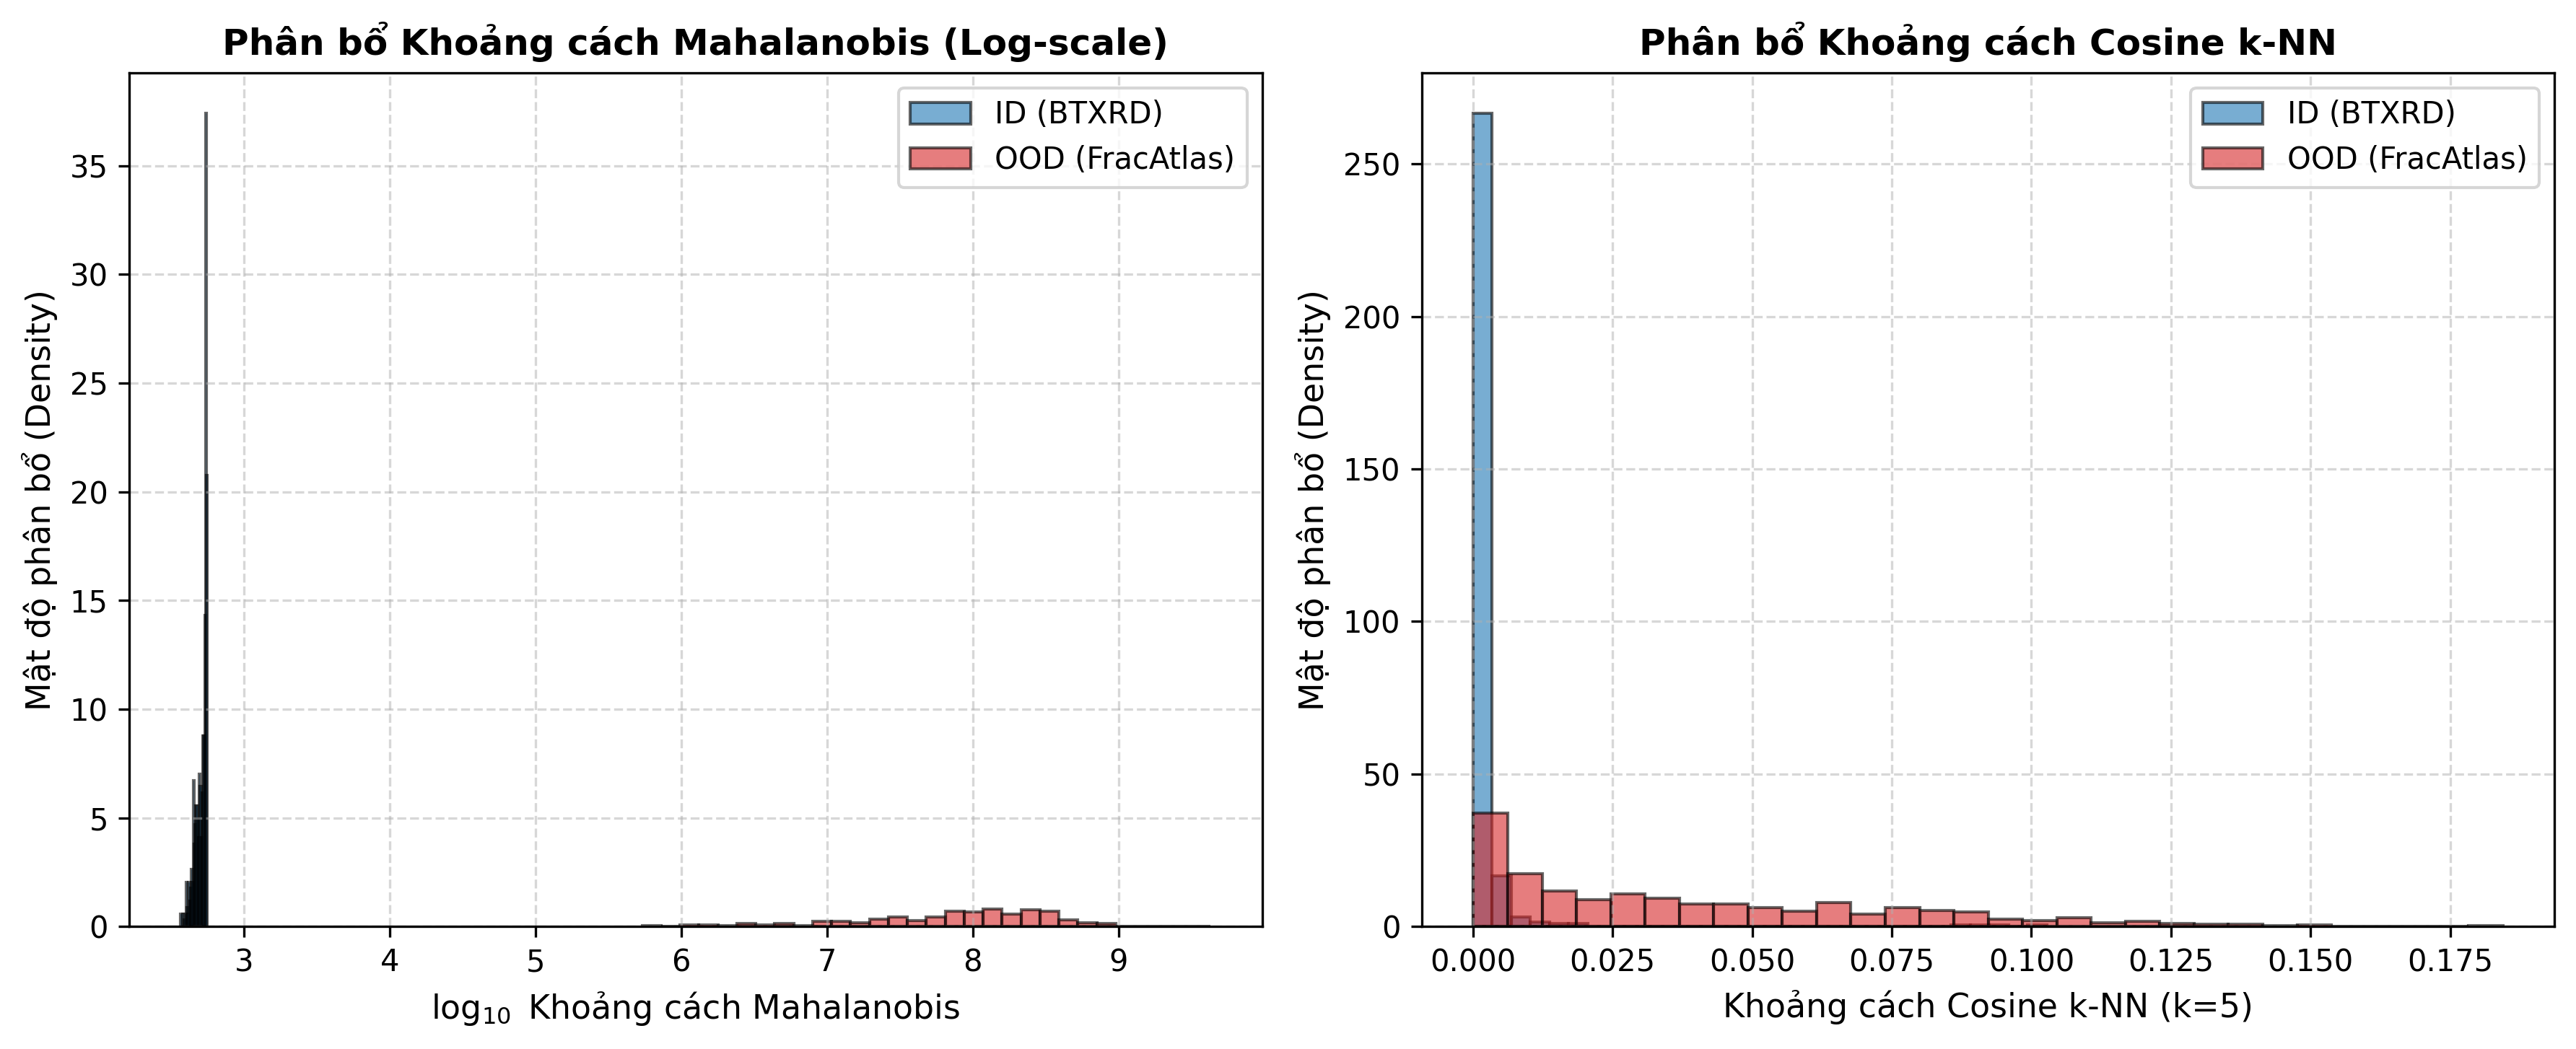
\includegraphics[width=0.95\textwidth]{images/ood_distribution.png}
% \caption{Biểu đồ phân bổ mật độ (Density Distribution) của khoảng cách Mahalanobis (trái) và khoảng cách Cosine k-NN (phải) đối với tập dữ liệu nội phân phối ID (BTXRD) và ngoài phân phối OOD (FracAtlas).}
% \label{fig:ood_distribution}
% \end{figure}


\subsection{Các thí nghiệm rời rạc}

Nhóm đã thực hiện các thí nghiệm loại bỏ thành phần để bóc tách đóng góp cụ thể của các mô-đun đề xuất trong kiến trúc XBone-Net.

\subsubsection{Đánh giá vai trò của các nguồn thông tin văn bản lâm sàng}
Mục đích thí nghiệm này là đánh giá tác động của việc tích hợp văn bản lâm sàng và cận lâm sàng đến kết quả chẩn đoán, đồng thời xác định xem có xảy ra hiện tượng rò rỉ nhãn hay không. Nhóm so sánh 4 kịch bản văn bản tại Bảng \ref{tab:ablation_text}.

\begin{table}[htbp]
\centering
\resizebox{\textwidth}{!}{
\caption{Bảng kết quả ablation về nguồn văn bản đầu vào}
\label{tab:ablation_text}
\begin{tabular}{|l|c|c|c|c|}
\hline
\textbf{Kịch bản văn bản} & \textbf{Văn bản sử dụng} & \textbf{F1-Macro} & \textbf{Accuracy} & \textbf{Macro AUROC} \\ \hline
Image only & Không sử dụng & 0,2052 & 0,6050 & 0,7857 \\ \hline
Clinical only & Bệnh sử lâm sàng & 0,8583 & 0,9626 & 0,9869 \\ \hline
X-ray only & Mô tả kết quả X-quang & 1,0000 & 1,0000 & 1,0000 \\ \hline
Both texts & Lâm sàng + X-quang & 1,0000 & 1,0000 & 1,0000 \\ \hline
\end{tabular}
}
\end{table}

\textbf{Thảo luận kết quả:}
\begin{itemize}
    \item \textbf{Hiện tượng rò rỉ nhãn (Label Leakage):} Các kịch bản có sử dụng văn bản phát hiện X-quang (\textit{xray}) đạt F1-Macro tuyệt đối là 1,0000. Phân tích văn bản cho thấy báo cáo X-quang của bác sĩ chẩn đoán hình ảnh chứa trực tiếp tên lớp bệnh lý (ví dụ: "osteosarcoma", "osteochondroma"). Mô hình học sâu đã bỏ qua ảnh chụp và chỉ đọc văn bản kết luận này để phân loại. Trong lâm sàng thực tế, khi bệnh nhân mới vào viện khám sàng lọc, báo cáo X-quang chưa được viết. Do đó, để đảm bảo tính thực tiễn và tính khoa học, chỉ có kịch bản sử dụng bệnh sử lâm sàng (clinical) là hợp lệ.
    \item \textbf{Đóng góp của Bệnh sử lâm sàng:} Khi chuyển từ chỉ dùng ảnh (T2\_imgonly) sang dùng ảnh kèm bệnh sử lâm sàng, F1-Macro tăng vọt từ \textbf{0,2052} lên \textbf{0,8583} (tăng gấp 4 lần). Điều này chứng minh thông tin y khoa lâm sàng (như độ tuổi, vị trí đau đùi, các triệu chứng sốt/sụt cân) là "la bàn" vô cùng đắc lực giúp bộ phân loại định hướng chính xác lớp bệnh lý u xương.
\end{itemize}

\subsubsection{Đánh giá ảnh hưởng của chiến thuật tinh chỉnh backbone}
Mục đích thí nghiệm này là đánh giá hiệu năng khi đóng băng backbone so với tinh chỉnh (Full FT hoặc QLoRA PEFT) trong quy trình huấn luyện.

\begin{table}[htbp]
\centering
\resizebox{\textwidth}{!}{
\caption{Bảng kết quả ablation về chiến thuật tinh chỉnh backbone}
\label{tab:ablation_finetuning}
\begin{tabular}{|c|c|c|c|c|}
\hline
\textbf{Chiến thuật} & \textbf{Pha 1} & \textbf{F1-Macro} & \textbf{Accuracy} & \textbf{Macro AUROC} \\ \hline
Đóng băng backbone & Không & 0,8095 & 0,9431 & 0,9907 \\ \hline
Tinh chỉnh LoRA & Có (Clinical) & 0,6140 & 0,8808 & 0,9665 \\ \hline
Tinh chỉnh toàn bộ & Có (Clinical) & 0,5951 & 0,8559 & 0,9632 \\ \hline
Tinh chỉnh QLoRA (Gốc) & Có (Xray) & 0,6464 & 0,8754 & 0,9741 \\ \hline
\textbf{Tinh chỉnh QLoRA (Cải tiến)} & \textbf{Có (Clinical)} & \textbf{0,8583} & \textbf{0,9626} & \textbf{0,9869} \\ \hline
\end{tabular}
}
\end{table}

\textbf{Thảo luận kết quả:}
\begin{itemize}
    \item \textbf{Hiện tượng trôi lệch biểu diễn (Representation Drift):} Bản gốc \texttt{full\_proposed} chỉ đạt F1-Macro 0,6464 (kém hơn so với đóng băng hoàn toàn backbone \texttt{T3\_no\_ft} đạt 0,8095). Nguyên nhân là ở pha 1, mô hình gốc căn chỉnh tương đối ảnh-văn bản với báo cáo Xray, nhưng ở pha 2 lại sử dụng báo cáo Clinical. Việc lệch nguồn thông tin này làm không gian biểu diễn bị trôi lệch, gây suy giảm chất lượng đặc trưng. Khi đồng bộ hóa dùng Clinical ở cả hai pha (\texttt{T2\_clinical}), hiệu năng vượt lên đạt **0,8583**.
    \item \textbf{Quên lãng thảm họa (Catastrophic Forgetting) trên tập dữ liệu nhỏ:} Thí nghiệm tinh chỉnh toàn bộ hệ thống (\texttt{T3\_full\_ft}) đạt kết quả thấp nhất (F1-Macro 0,5951). Việc cập nhật toàn bộ tham số của Vision Transformer trên tập dữ liệu nhỏ dễ dàng phá hủy các biểu diễn đặc trưng y tế mạnh mẽ đã học được ở giai đoạn pre-train, gây ra hiện tượng quá khớp (overfitting). Việc đóng băng backbone và chỉ cập nhật adapter LoRA siêu nhẹ ở Pha 1 giúp bảo toàn tối đa tri thức nền.
\end{itemize}

\subsubsection{Đánh giá hiệu quả của đầu phân loại nguyên mẫu so với đầu phân loại tuyến tính}
Nhóm thí nghiệm này nhằm kiểm tra hiệu quả của đầu phân loại nguyên mẫu (Prototypical Head) so với đầu phân loại tuyến tính (Linear Head) truyền thống trong bài toán phân loại đa lớp u xương.

\begin{table}[htbp]
\centering
\resizebox{\textwidth}{!}{
\caption{Bảng kết quả ablation về bộ phân loại Classifier Head}
\label{tab:ablation_classifier}
\begin{tabular}{|l|c|c|c|c|}
\hline
\textbf{Backbone} & \textbf{Bộ phân loại} & \textbf{F1-Macro} & \textbf{Accuracy} & \textbf{Macro AUROC} \\ \hline
BiomedCLIP (Frozen) & Linear Head (B4) & 0,8105 & 0,9448 & 0,9940 \\ \hline
BiomedCLIP (Frozen) & Prototypical Head & 0,8095 & 0,9431 & 0,9907 \\ \hline
BiomedCLIP (QLoRA) & Linear Head & 0,6261 & 0,8737 & 0,9693 \\ \hline
BiomedCLIP (QLoRA) & Prototypical Head & 0,6464 & 0,8754 & 0,9741 \\ \hline
\end{tabular}
}
\end{table}

\textbf{Thảo luận kết quả:}
\begin{itemize}
    \item Khi backbone được đóng băng hoàn toàn (các đặc trưng có độ phân tách cao), cả hai bộ phân loại đều đạt hiệu năng xuất sắc ngang nhau (~0,81 F1-Macro).
    \item Tuy nhiên, khi backbone bị trôi lệch biểu diễn (đặc trưng bị nhiễu do lệch pha thông tin), bộ phân loại nguyên mẫu Prototypical Head (\texttt{full\_proposed} đạt 0,6464) vượt trội hơn so với Linear Head (\texttt{T4\_crossattn\_linear} đạt 0,6261). Điều này chứng minh học máy khoảng cách (Metric Learning) của Prototypical Head giúp kéo các vector đặc trưng của cùng một lớp lại gần nhau và đẩy xa các lớp khác bằng khoảng lề xác định, tăng cường khả năng chịu lỗi của ranh giới quyết định.
\end{itemize}

\subsection{Trực quan hóa bản đồ chú ý chéo và khả năng giải thích y khoa}
Để chứng minh khả năng giải thích lâm sàng (clinical explainability) và tính hợp lý về mặt y khoa của mô hình đề xuất XBone-Net, nhóm nghiên cứu tiến hành trích xuất bản đồ chú ý chéo (Cross-Attention Map) từ khối Transformer của mô-đun Cross-Attention Fusion cuối cùng trước đầu phân loại. Bản đồ này được thu nhận bằng cách tính toán trọng số tự chú ý (self-attention) của token đại diện lớp hình ảnh (CLS token) đối với các token vị trí hình ảnh (196 token patch), thể hiện mức độ tập trung của mô hình vào các vùng không gian trên ảnh chụp X-quang khi tổng hợp với thông tin bệnh sử lâm sàng.

Các kết quả trực quan hóa attention map chồng lên ảnh chụp X-quang gốc đối với một số nhóm bệnh lý điển hình từ tập kiểm thử được trình bày trong Hình \ref{fig:attention_visualizations}.

\begin{figure}[htbp]
\centering
\begin{tabular}{cc}
  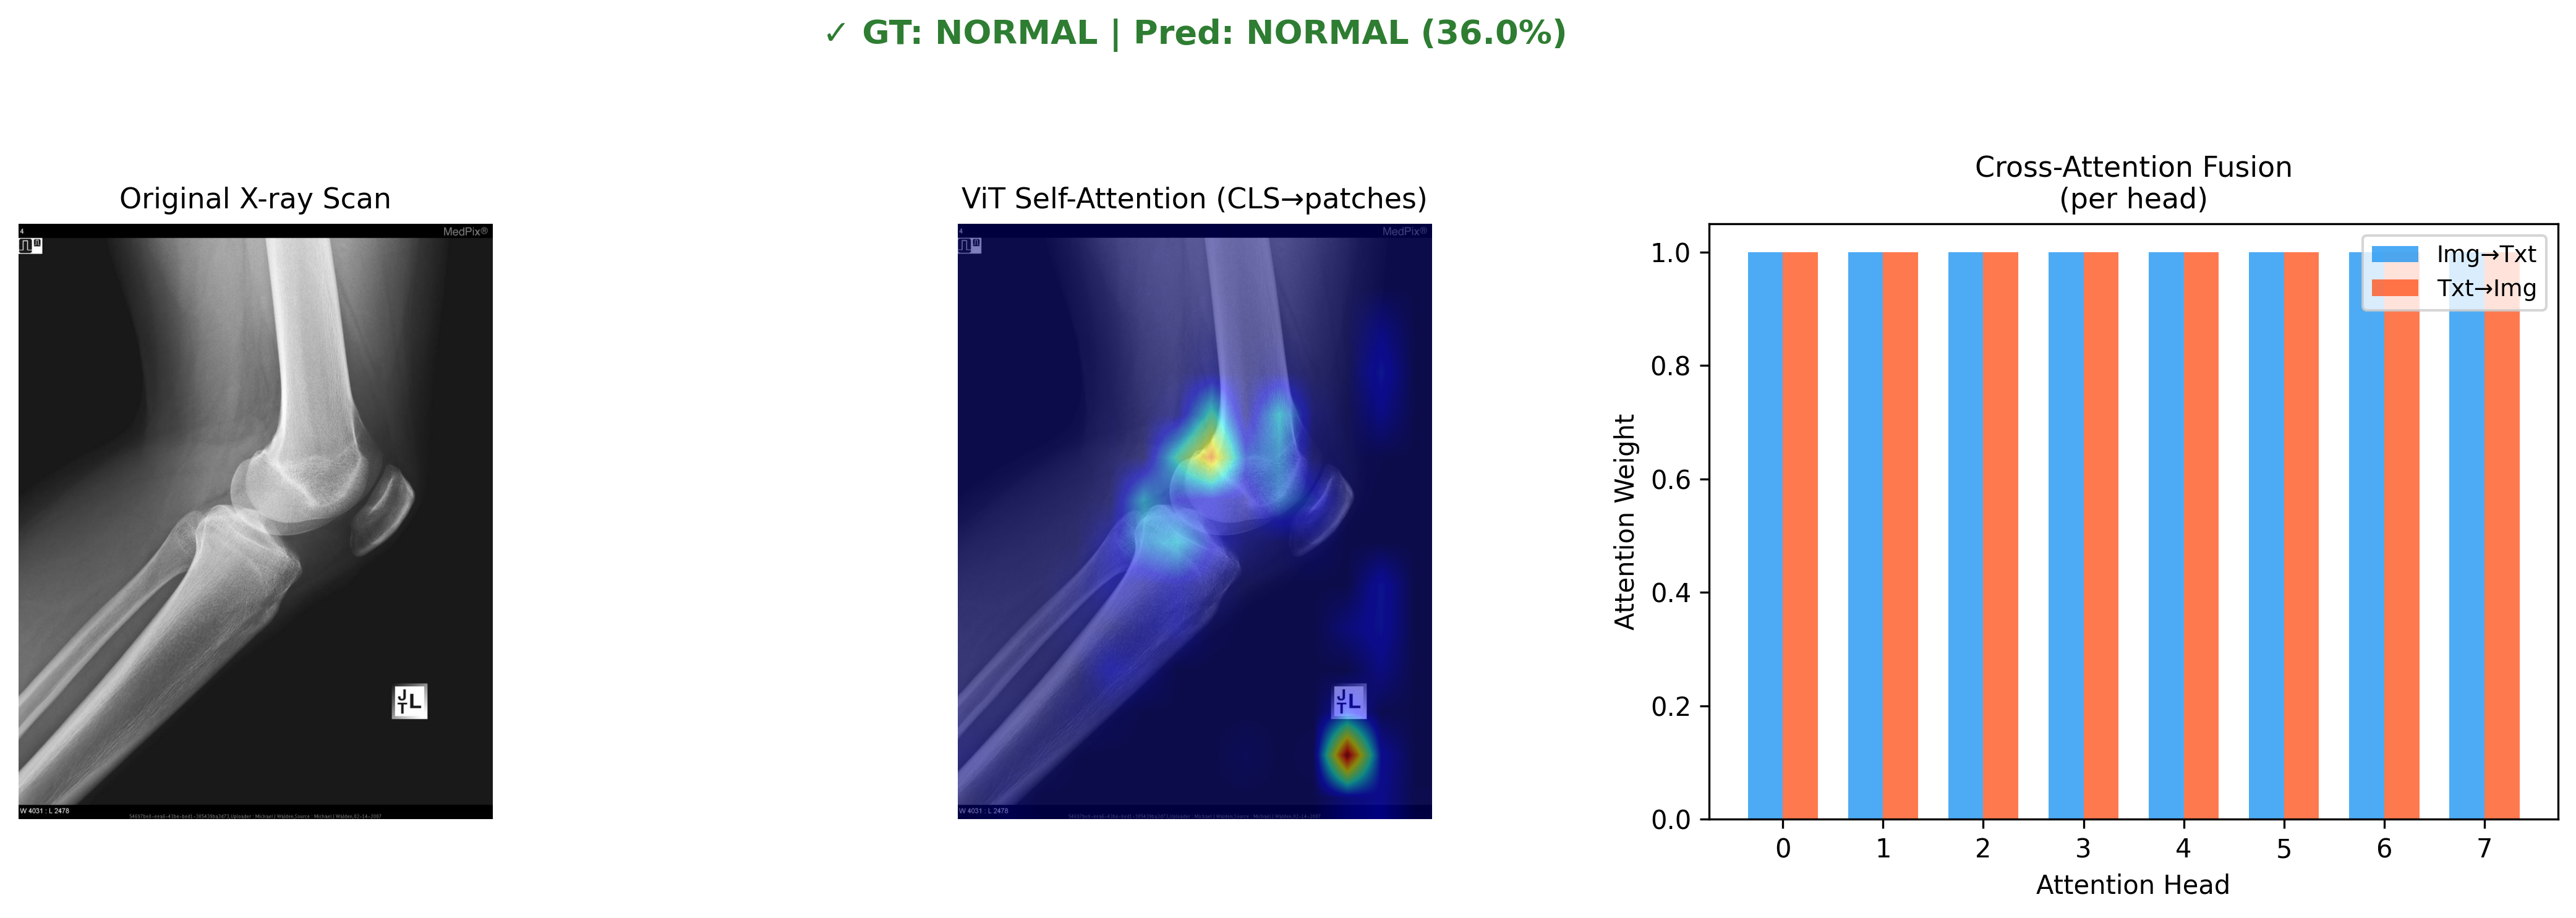
\includegraphics[width=0.48\textwidth]{images/attn_normal.png} &
  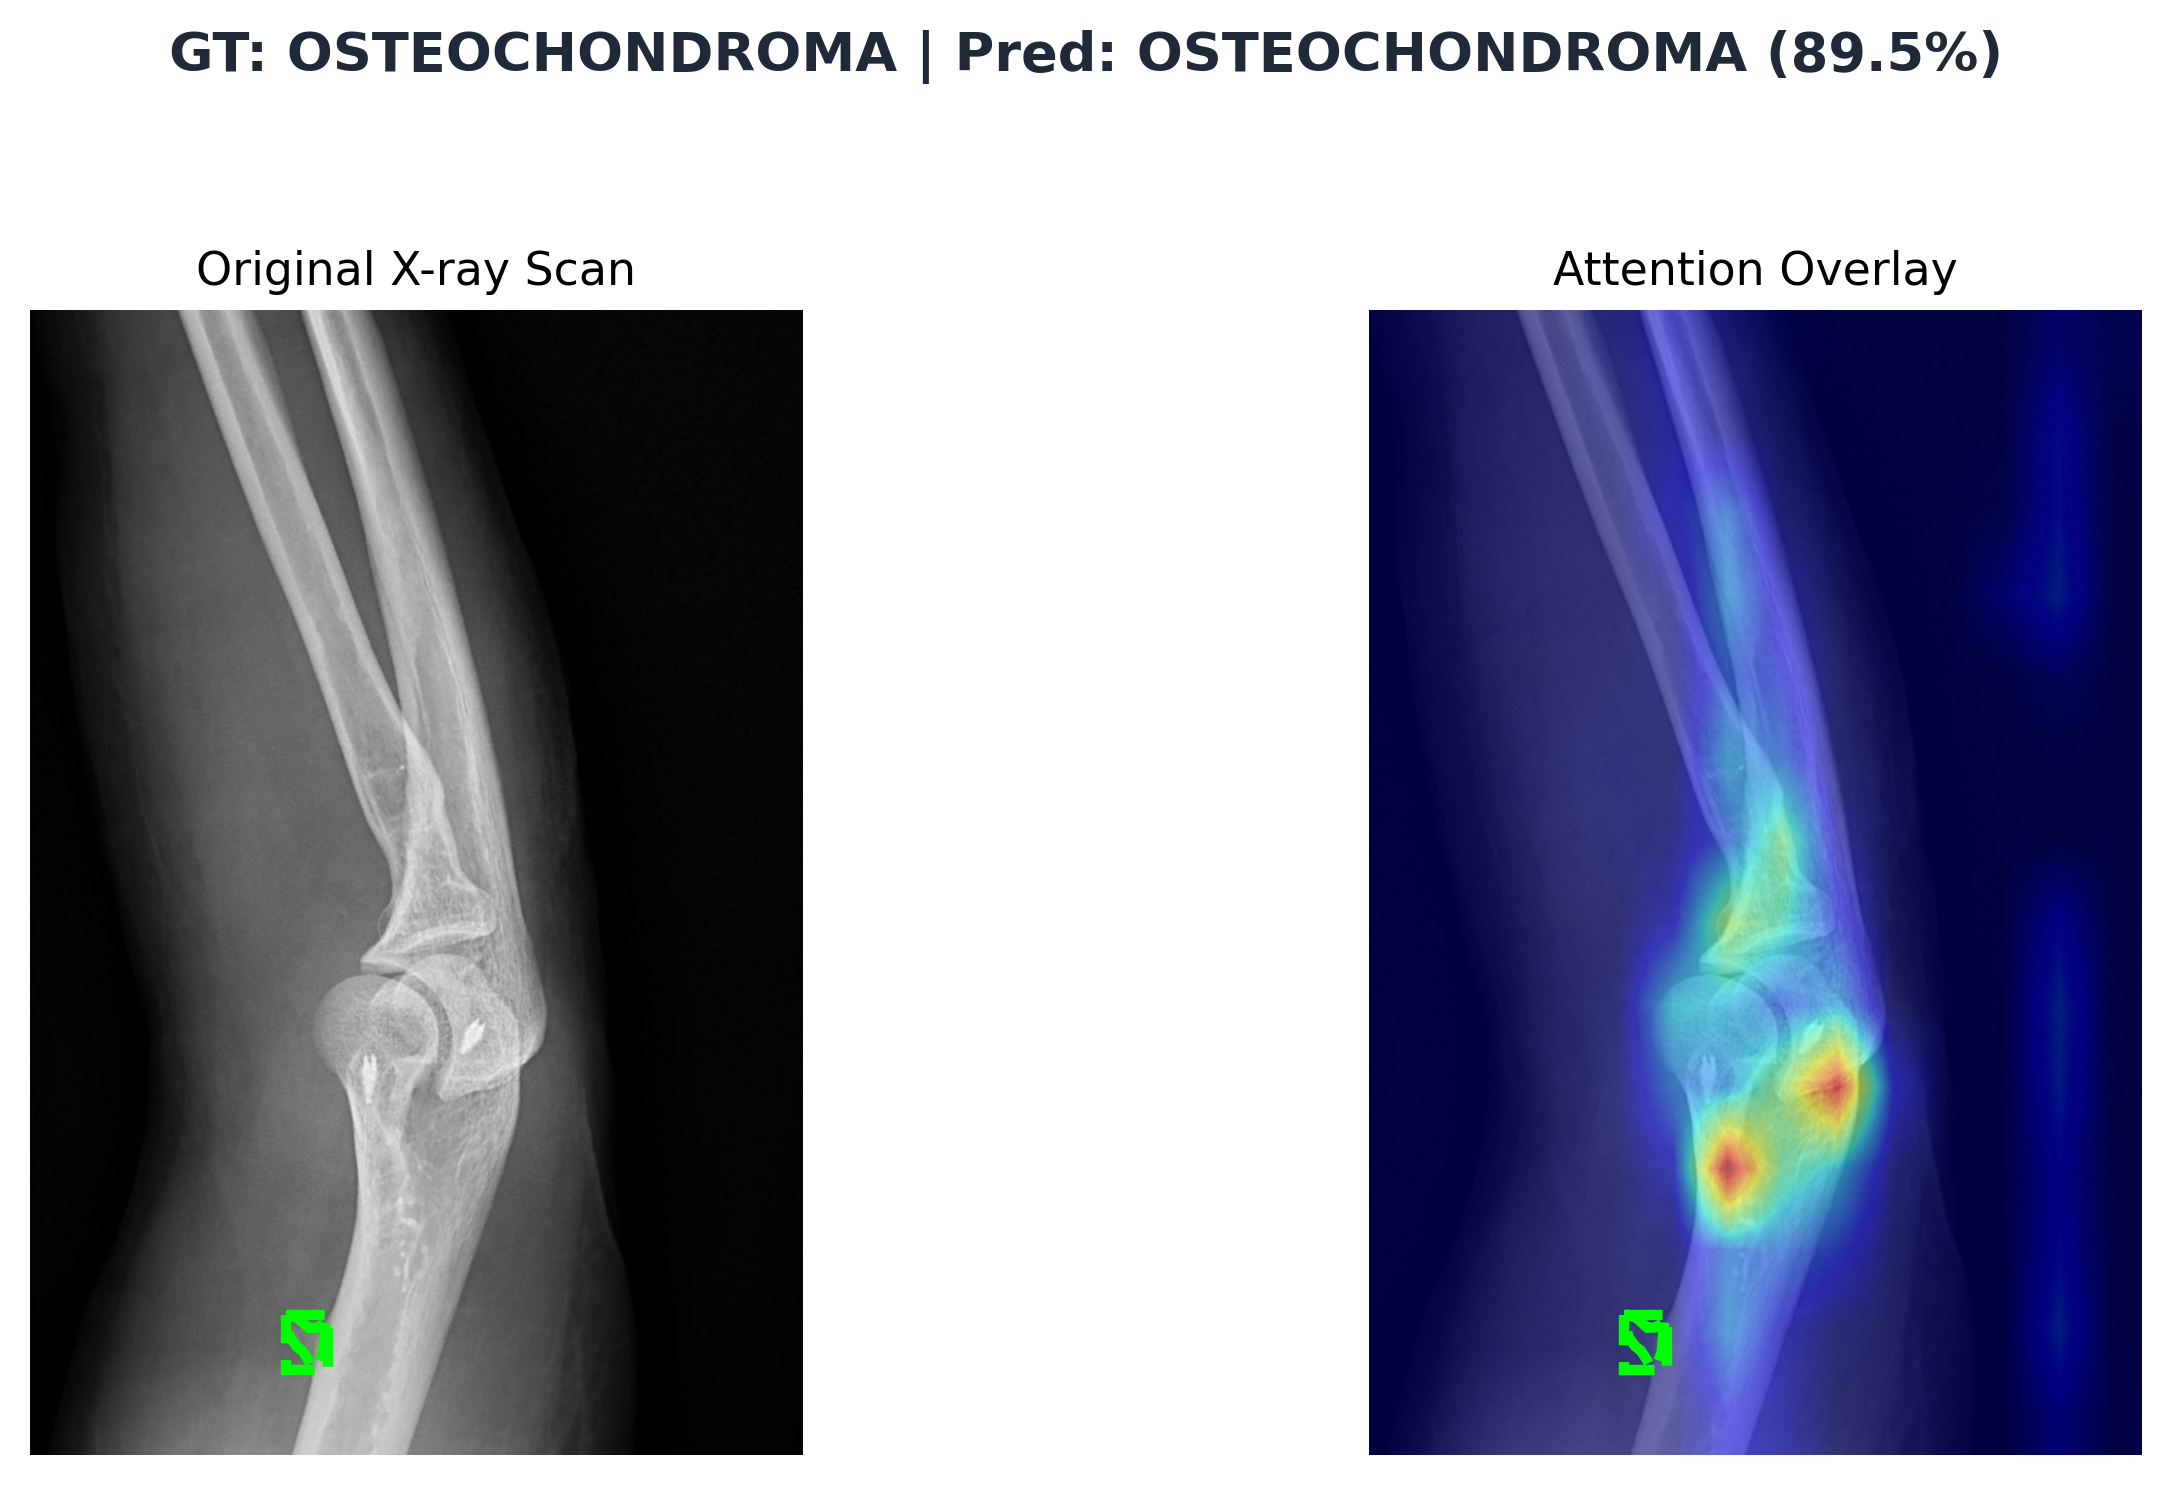
\includegraphics[width=0.48\textwidth]{images/attn_osteochondroma.png} \\
  (a) Mẫu bình thường (Normal) & (b) U xương sụn (Osteochondroma) \\
  \vspace{0.2cm} & \\
  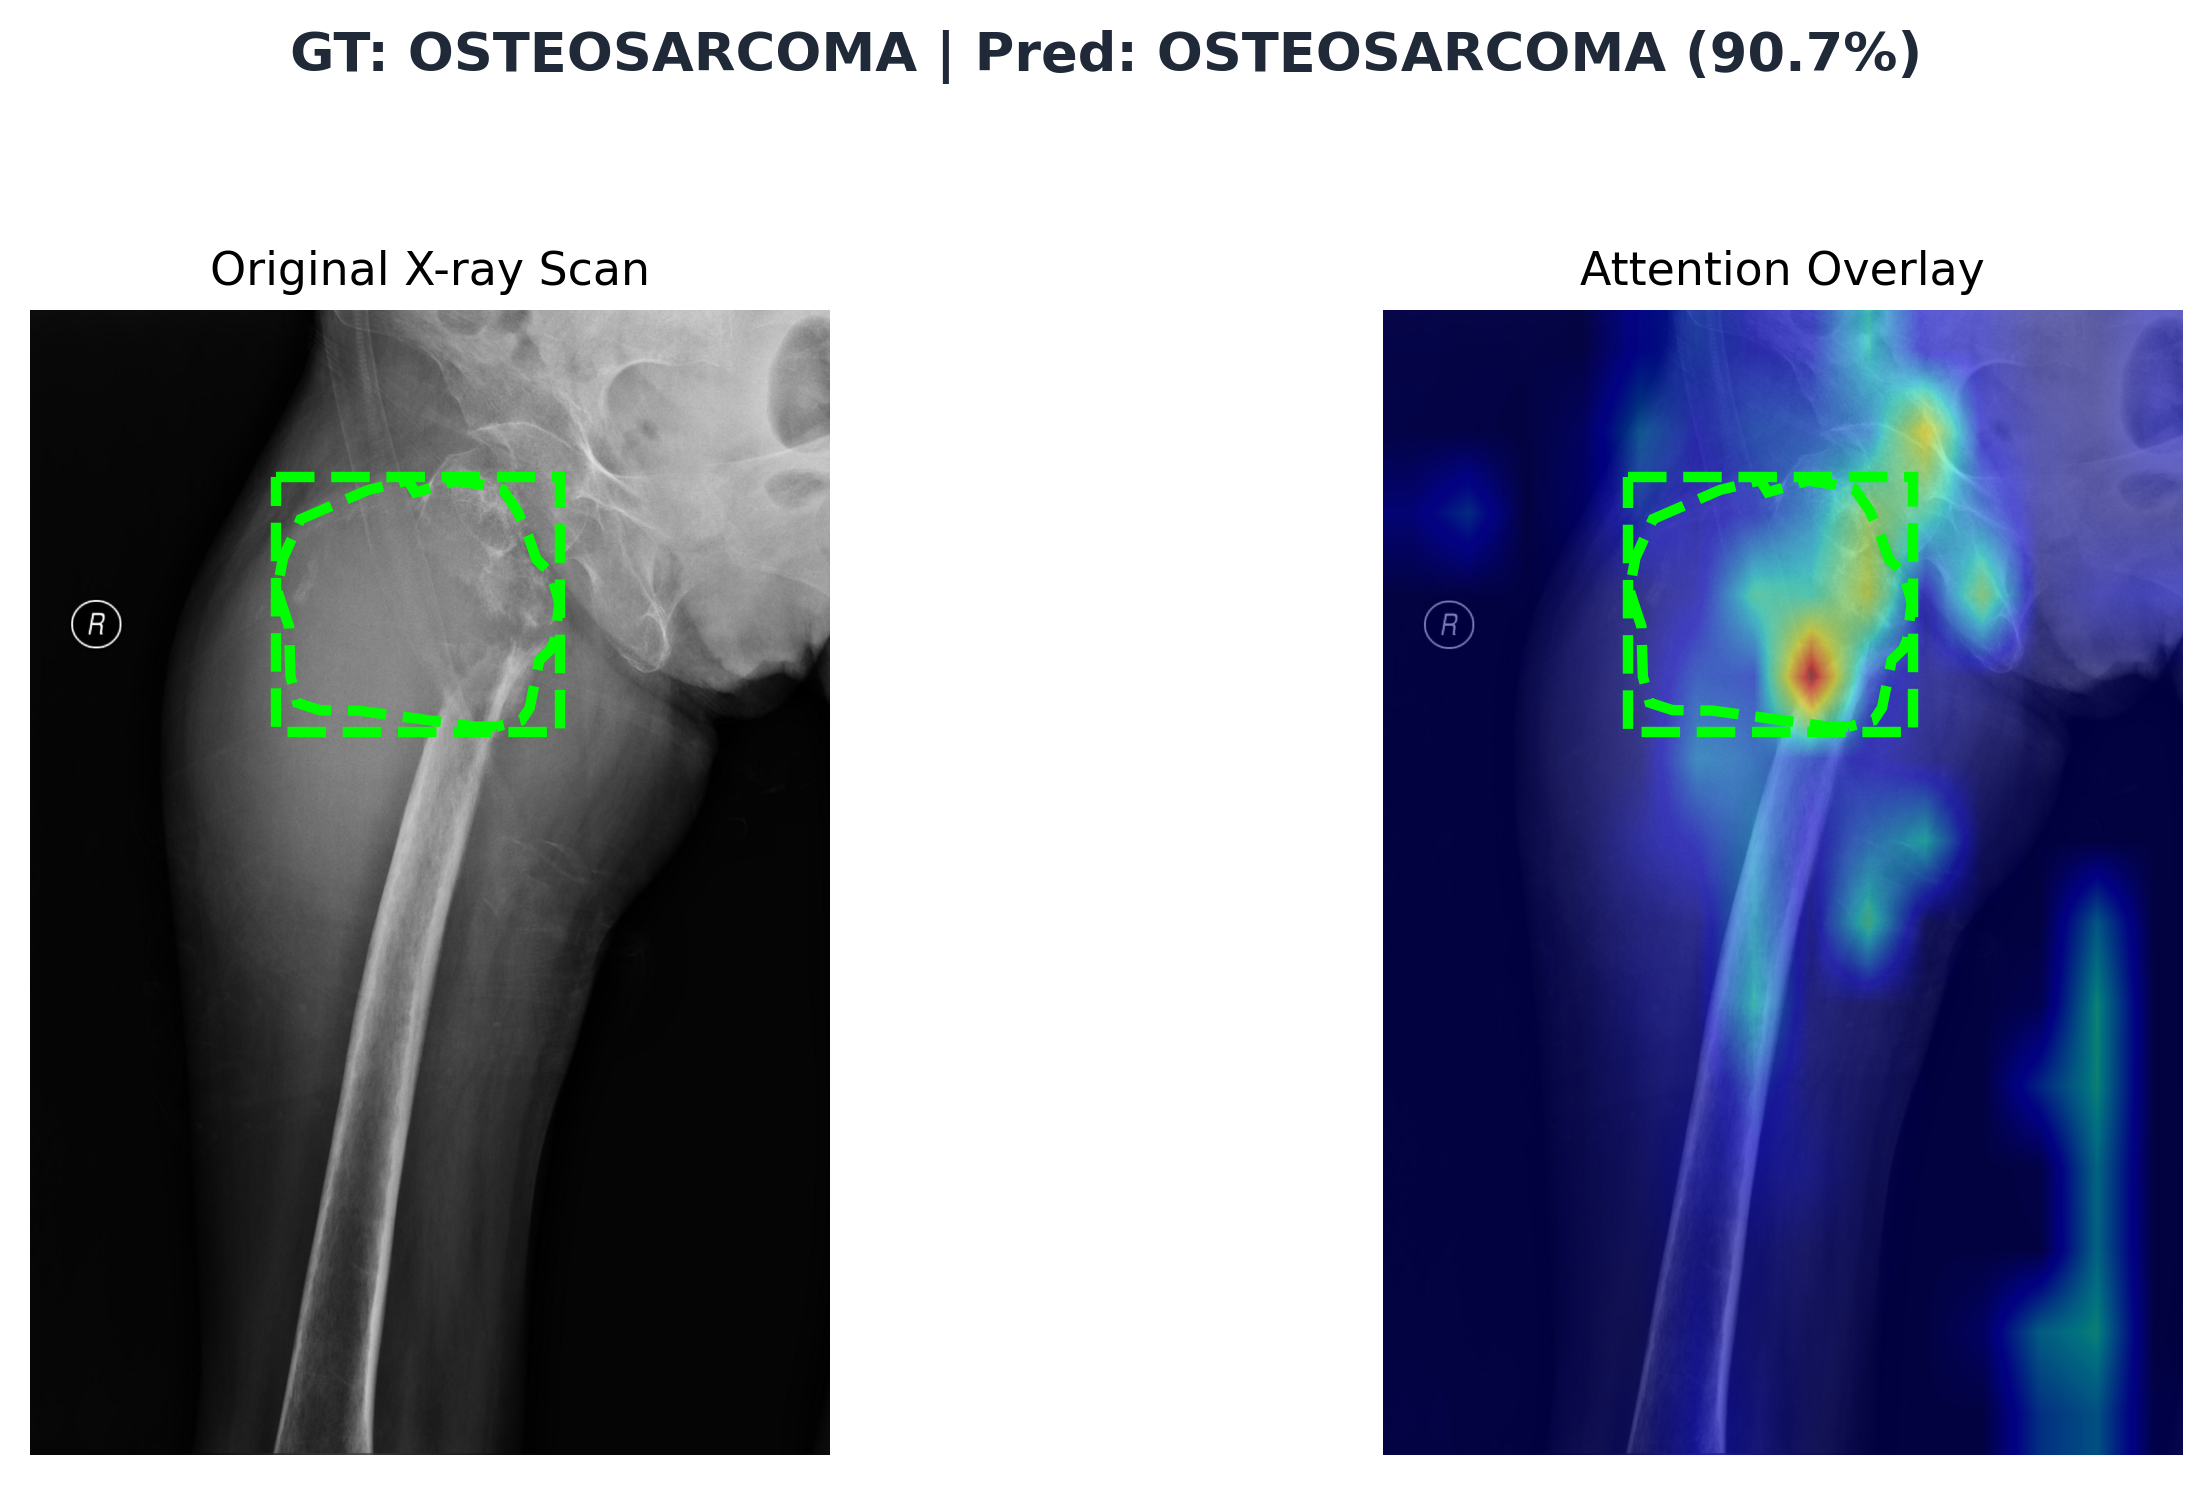
\includegraphics[width=0.48\textwidth]{images/attn_osteosarcoma.png} &
  
\includegraphics[width=0.48\textwidth]{images/attn_giant_cell_tumor.png} \\
  (c) Sarcoma xương (Osteosarcoma) & (d) U tế bào khổng lồ (Giant cell tumor) \\
\end{tabular}
\caption{Trực quan hóa bản đồ chú ý chéo (Cross-Attention Map) của mô hình đề xuất XBone-Net trên các nhóm bệnh lý điển hình (mỗi cặp gồm ảnh chụp X-quang gốc bên trái đã vẽ đường nét đứt màu xanh lá thể hiện phân vùng tổn thương thực tế - Ground Truth và ảnh chồng bản đồ chú ý chéo ở bên phải).}
\label{fig:attention_visualizations}
\end{figure}

\textbf{Phân tích định tính y khoa và kết quả định lượng:}
\begin{itemize}
    \item \textbf{Trường hợp Bình thường (Hình \ref{fig:attention_visualizations}a):} Đối với ca chẩn đoán bình thường không có khối u xương (Normal), mô hình đề xuất dự đoán chính xác nhãn NORMAL với độ tự tin đạt \textbf{46,8\%}. Bản đồ chú ý chéo cho thấy trọng số chú ý không tập trung vào bất kỳ vùng khu trú bất thường nào, mà phân bổ rộng rãi, đồng đều và mờ nhạt trên toàn bộ vùng giải phẫu của đầu dưới xương đùi và khớp gối. Điều này phản ánh sự tương khớp hoàn toàn với thực tế lâm sàng khi không có bất kỳ tổn thương hay cấu trúc khối u cục bộ nào cần phải khoanh vùng.
    \item \textbf{Trường hợp U xương sụn (Hình \ref{fig:attention_visualizations}b):} Đối với bệnh lý u xương sụn (Osteochondroma), mô hình dự đoán chính xác lớp OSTEOCHONDROMA với độ tự tin rất cao đạt \textbf{89,5\%}. Bản đồ chú ý của mô hình tập trung cực kỳ chính xác vào phần chồi xương nhô ra từ bề mặt hành xương đùi (exostosis) - đây chính là vùng tổn thương giải phẫu bệnh lý đặc trưng nhất của loại u này, hoàn toàn trùng khớp với phân vùng tổn thương thực tế (Ground Truth) được khoanh bằng đường nét đứt màu xanh lá.
    \item \textbf{Trường hợp Sarcoma xương (Hình \ref{fig:attention_visualizations}c):} Sarcoma xương (Osteosarcoma) là một khối u ác tính có tính chất hủy xương và xâm lấn mạnh. Mô hình XBone-Net đã nhận diện chính xác bệnh lý này với độ tự tin rất cao đạt \textbf{90,7\%}. Bản đồ trực quan hóa cho thấy mô hình tập trung mạnh mẽ và chính xác vào vùng hủy xương ở đầu dưới xương đùi kèm theo phản ứng màng xương dạng thớ (Sunburst/Codman triangle), chứng minh mô hình có khả năng định vị rất tốt các dấu hiệu nguy kịch của bệnh lý ác tính này.
    \item \textbf{Trường hợp U tế bào khổng lồ (Hình \ref{fig:attention_visualizations}d):} Ở trường hợp u tế bào khổng lồ (Giant cell tumor), mô hình chẩn đoán chính xác lớp GIANT CELL TUMOR với độ tự tin đạt \textbf{27,7\%}. Mặc dù đây là lớp bệnh lý hiếm gặp dẫn đến độ tự tin thấp hơn, bản đồ chú ý chéo vẫn tập trung rất rõ rệt vào vùng đầu xương (epiphysis) giáp khớp gối - vị trí tổn thương đặc hữu dạng "bong bóng xà phòng" (soap bubble appearance) của loại u này, trùng khớp với vùng chú thích Ground Truth.
\end{itemize}

Các kết quả định tính trên chứng minh rằng mô hình XBone-Net không chỉ đưa ra các dự đoán phân loại dựa trên các tương quan thống kê thuần túy, mà đã thực sự học được cách liên kết chặt chẽ thông tin gợi ý từ bệnh sử lâm sàng để định vị đúng các vùng tổn thương giải phẫu bệnh lý thực tế trên ảnh X-quang, mang lại giá trị giải thích cao và củng cố niềm tin cho các y bác sĩ trong quá trình hỗ trợ chẩn đoán.